\documentclass{article}
\usepackage{url}
\usepackage{fullpage}
\usepackage{graphicx}
\usepackage{subcaption}
\usepackage[utf8]{inputenc}
\begin{document}
\title{Let's build electrostatic headphones}
\author{Arno Mayrhofer \and Benedikt Becsi}
\maketitle

\tableofcontents

\newpage

\section{Introduction}
\label{s:intro}
The following document will describe the journey to construct your own electrostatic headphones starting with zero, zilch, nada, niente and nichts. In Section \ref{s:tools} we will list the tools required for the building process, which will be followed by a list of materials in Section \ref{s:materials}. The actual construction process is split into five parts, the building of the driver (Section \ref{s:driver}), enclosure (Section \ref{s:driver}), headband (Section \ref{s:headband}) and earpads (Section \ref{s:pads}) with a final assembly in Section \ref{s:assembly}. Finally, the last two chapters will deal with measurements (Section \ref{s:measurements}) and things that we would do differently for the second pair (Section \ref{s:future}).

The whole construction is based on the Head-Fi.org thread \cite{head-fi-diy-thread}, with different and more detailed sources (\cite{electrostatic-hp-design,tcengineering-electrostatic-drivers,ww_1979}) given in the respective sections.

\begin{figure}[htb]
    \centering
    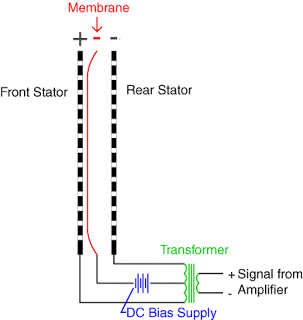
\includegraphics[width=0.5\textwidth]{images/esl_animation.png}
    \caption{Electrical concept}
    \label{f:intro:e-concept}
\end{figure}

The basic electrical concept of a electrostatic headphone can be seen in Fig. \ref{f:intro:e-concept}. An amplifier provides an input signal that is then transformed to yield the desired output voltage that drives the two stators. Additionally, there is a negative DC current that keeps the diaphragm charged.

\section{Required tools}
\label{s:tools}

To build the drivers it is highly recommended that you have access to a good CNC machine. Since we didn't have one of those standing around, we looked for a so called fablab, i.e. a community led workshop for creative projects. We eventually ended up at the Viennese Metalab\footnote{\url{https://metalab.at/}} which gave us access to a heavy duty level CNC machine and an introduction on how to use it by Sebastian Bachmann\footnote{\url{https://www.reox.at/}}, which eased the learning curve significantly. The principal introduction included instructions on how to set up, start and operate the machine and the control terminal, as well as some GGode basics (the programming language that controls the machine's behaviour - more on that in section \ref{s:driver:design:gcode}). Most importantly, as it can be potentially quite dangerous to operate one of those things, it covered security basics, which is definitely the first starting point for anyone new to CNC. Don't skip your tutorial lessons, kids!

Since you might be interested in the budget needed for this, it of course depends on the lab's membership policy - most labs we found had a monthly fee with a minimum subscription period, but we were able to come to an arrangement with a voluntary contribution without binding membership. Most people running those kinds of open creative space are pretty chill, so don't be afraid to ask!

If you can't find a place or plan to work on more DIY-projects in the future, it might be worth it to purchase a CNC mill for yourself or with a group of like-minded people. It's amazing what's going on in the field of affordable, small-scale, DIY and hobby-use CNC in the last couple of years. Here are some links if you're more interested in a purchase:\\
\url{https://www.millrightcnc.com/product-page/millright-cnc-m3-kit-bundle}\\
\url{http://www.makerdreams.it/}\\
\url{https://www.sorotec.de/shop/}\\
\\
Also, some labs require you to buy the wearout parts yourself. You can get CNC tools here:\\
\url{http://cnc-plus.de/}\\
\url{https://www.sorotec.de/shop/}\\
\\
An electric drill was used for the assembly screws and headband construction. The earpads were sewn from hand and as such only thread and needle was required for that. The step up transformer that we built to drive the headphones required a basic electronics lab and in particular a soldering station.

\section{Required materials}
\label{s:materials}
In this section we list all the materials we had to purchase for the headphones and our DIY step-up transformer. We provide you with the links where we bought the materials, but depending on where you live you might find better suppliers yourself.

\begin{enumerate}
    \item 1 mm PCB FR-4 for stators and dust protection spacers:  \footnote{\url{https://www.conrad.com/ce/en/product/523656/PCB-material-Photo-coating-positive-single-sided-35-m?ref=list}}
    \item 0.5 mm PCB for spacers: \footnote{\url{https://www.conrad.com/ce/en/product/523630/PCB-material-Photo-coating-positive-single-sided-35-m?ref=list}}
    \item 3 $\mu m$ Mylar (for diaphragm): \footnote{\url{https://www.ebay.com/itm/Electrostatic-Speaker-Membrane-Dupont-Mylar-C-3um-40M/172781729300?epid=666335680&hash=item283a97f614:g:jg0AAOSwrklVPe61}} (with that, you should have all your mylar needs covered for years to come!)
    \item 1 $\mu m$ Mylar (for dust protection): \footnote{\url{https://www.freeflightsupplies.co.uk/index.php/products/lightweight-covering-materials}}
    \item Anti-static display cleaner for diaphragm coating: \footnote{\url{https://www.conrad.com/ce/en/product/995207/DataFlash-DF1620-Content-250-ml?ref=searchDetail}}
    \item Acrylic spray for insulating the stators: \footnote{\url{https://www.conrad.com/ce/en/product/1198455/Acrylic-paint-Revell-Black-matt-08-Spray-can-100?ref=searchDetail}}
    \item Thin and stretchy artificial leather for the earpads and headband (should be available in a textile shop)
    \item Wood for the enclosure and headband, several boards with 4mm and 10mm thickness; we used lime and spruce
    \item Metal rods (3mm welding rods) for the headband
    \item 3 cm acoustic foam (pads and headband)
    \item Cable plus connectors
    \item Screws for the assembly (2,5 x 20 mm)
    \item Clear varnish or glaze for wood finish
    \item Two-component glue: \footnote{\url{https://www.conrad.com/ce/en/product/478703/UHU-Plus-Schnellfest-Two-component-adhesive-45700-35-g?ref=list}}
    \item Contact glue for gluing the membrane to the stators and the earpads: \footnote{\url{https://www.conrad.com/ce/en/product/631802/UHU-greenit-Contact-adhesive-45401-650-g?ref=searchDetail}}

\end{enumerate}
Head-fi.org \footnote{\url{http://www.head-fi.org/t/826032/electrostatic-ear-speaker-diyers-suppliers-list}} has a more comprehensive list of material suppliers.
\\
\\
Materials needed for the amplifier:
\begin{enumerate}
    \item 4 Audio transformers 6V - 230V (OEP N35A002F) \footnote{\url{https://uk.rs-online.com/web/p/audio-transformers/2106475/}}
    \item 1 Power transformer 230V - 230V (Triad Magnetics FP230-25) \footnote{\url{https://eu.mouser.com/search/ProductDetail.aspx?r=553-FP230-25}}
    \item 2 1 Ohm wirewound resistors \footnote{\url{https://eu.mouser.com/search/ProductDetail.aspx?r=71-RS0101R000FE73}}
    \item 6 1kV diodes \footnote{\url{https://eu.mouser.com/search/ProductDetail.aspx?r=625-RGP10M-E3}}
    \item 2 10 MOhm resistors \footnote{\url{https://eu.mouser.com/search/ProductDetail.aspx?r=594-SFR25H0001005JR5}}
    \item 6 10 nF capacitors \footnote{\url{https://eu.mouser.com/search/ProductDetail.aspx?r=75-564R30GAS10}}
    \item 1 3.9 kOhm resistor \footnote{\url{www.aliexpress.com}}
    \item Power cord plus plug
    \item Cables
    \item Test circuit board
\end{enumerate}

\section{Building the driver}
\label{s:driver}

\subsection{Design of the stators and spacers}
\label{s:driver:design}
In the following the stators and spacers will be designed and the designs will be prepared for CNC milling. As the stators and spacers are 2-D, we decided to use Inkscape \footnote{\url{https://www.inkscape.org}} for our design purposes. There are plenty of guides on how to use Inkscape around so we assume that the reader is familiar with it. But in the end we almost exclusively used the basic objects like spheres and ellipses and boolean operators (to be found under the \textit{Path} menu).

\begin{figure}
    \centering
    \begin{subfigure}[b]{0.24\textwidth}
        
\includegraphics[width=\textwidth]{images/stator.png}
        \caption{Stator}
        \label{f:driver:stator}
    \end{subfigure}
    \begin{subfigure}[b]{0.24\textwidth}
        
\includegraphics[width=\textwidth]{images/spacer_front.png}
        \caption{Front spacer}
        \label{f:driver:spacer_front}
    \end{subfigure}
    \begin{subfigure}[b]{0.24\textwidth}
        
\includegraphics[width=\textwidth]{images/spacer_back.png}
        \caption{Back spacer}
        \label{f:driver:spacer_back}
    \end{subfigure}
    \begin{subfigure}[b]{0.24\textwidth}
        
\includegraphics[width=\textwidth]{images/spacer_dust.png}
        \caption{Spacer for dust protector}
        \label{f:driver:spacer_dust}
    \end{subfigure}
    \caption{All PCB driver components}
    \label{f:driver:components}
\end{figure}

In general the ellipse which contains all driver components is 130 mm high and 94 mm wide. The inner ellipse that determines the active area is 110 mm high and 74 mm wide. The holes drilled into the stator only cover this active area and are laid out such that approximately 40\% of the active area is open, i.e. covered by holes. The distance between the holes is 0.8421 mm in vertical and 0.88 mm in horizontal direction and each hole has a diameter of 2 mm. To generate such a tiled array of holes in Inkscape draw one hole and then use the \textit{Create tiled clones} option that can be found under \textit{Edit - Clone}. The holes outside the active are where removed manually. The resulting stator can be seen in Fig. \ref{f:driver:stator}. A total of four stators need to be milled from 1mm FR4 PCB. The eight cut-outs that are present in each driver component were designed to allow easier screw insertion in the enclosing. It turned out though that we only needed four screws in the end and it would have been possible to work without those cut-outs at all. At the bottom of the components there is a varying number of half-circle cut-outs. These ensure that cables can be connected at other components and provide insulation to the present one. The front and back stator seen in Fig. \ref{f:driver:spacer_front} and Fig. \ref{f:driver:spacer_back} are made from 0.5 mm FR4 PCB. The dust spacer in Fig. \ref{f:driver:spacer_dust} is made from 1 mm PCB. Each spacer needs to be produced twice, one for each side.

A few general design guidelines that we found on the head-fi thread indicated the following. The diameter of the holes (2 mm in our case) should not be larger than the distance from stator to spacer. The reason for not having the holes cover the whole stator is that this increases the stability of the stator. A large diaphragm size is quite important as this improves low frequency response. Obviously, if the open area becomes too large then the diaphragm will be too flexible and touch the stators which will cause it to discharge. Because of this the ratio of spacer thickness to diaphragm width should not be larger than 1:120. If this ratio is very large a lower bias voltage can be used to avoid the membrane touching the stators.

All \textit{*.svg} files that are used for the CNC milling can be found in the \textit{resources.zip} which can be found on github.com\footnote{\url{https://github.com/Azrael3000/headphone-guide/raw/master/resoures.zip}}.

%Diameter of the holes (2mm) should not be larger than the distance from stator to spacer. The holes in the stator should not cover the whole stator. Instead there should be a perimeter that acts as an air damper and avoids resonance frequencies in the upper midrange or lower treble. The size of the diaphragm is quite important as low frequencies require a large diaphragm surface. The active area should have a diameter of about 80 mm. The ratio of spacer thickness to diaphragm width should not be larger than 1:120 to avoid contact between stator and diaphragm. Lowering the bias voltage can help with very large ratios. Open area of the stators should be around 40\% in order to avoid issues with stability of the stator.

%When drilling holes on the stator the feed rate should be at around 3600 mm/min.  For routing and cutting, it should be slowed down to around 1800 - 2400 mm/min.
%
%In order to protect the diaphragm a dust and sweat protection needs to be used. This dust cover will be made from crumpled Mylar and will be located on the same side as the coating of diaphragm.
%
%\url{http://www.head-fi.org/t/498292/my-diy-electrostatic-headphones/660#post_8897170} -> Design pictures of the Orpheus clones; apparently this design lacks some bass punch, maybe increase non-holed perimeter for improvements? Later on it is proposed to decrease the width a bit to improve stability. This would yield the dimensions of 110 x 74 mm (open area of 104 x 74 mm of orpheus clone).
%
%\url{http://www.head-fi.org/t/498292/my-diy-electrostatic-headphones/1155#post_10142154} -> potential improvement of stability by making a hole in the center of the stators (one additional advantage: it's easier to detect issues with the diaphragm as it can be examined visually)
%
%The edges of the spacers need to be sanded down a bit in order to avoid copper dust on the sides and spurious electrical contacts. Holes should be de-burred from copper.
%
%Do not mirror the stators so that the drilling always goes away from the diaphragm (drill pushes small bits of material on the outside) TODO REPHRASE
%
%Inner ellipse: 55 x 37, outer: 65 x 47. Radius of holes: 1mm, multiplicator: 39 in x and 26 in y direction with distance 0.8421 and 0.88 in those directions, respectively.

\subsubsection{Gcode creation}
\label{s:driver:design:gcode}

After creating the \textit{*.svgs} with the outline of all shapes the next step is to produce Gcode, i.e. the instructions for the CNC machine that can be understood by it. Note that we were using a CNC machine that was using LinuxCNC and it pretty much understood the Gcode produced by the tool presented in the following. The first important step is to create a milling strategy. For all FR4 parts (stators and spacers) we decided to use double sided tape to glue the FR4 boards to a flat piece of scrap wood. This means that all paths will be cut 0.2mm deeper than the FR4 thickness. This ensures that the milling is deep enough and only leaves some scratches on the scrap wood.

Before we start with the Gcode creation we need to decide on which drills and end mills to use. Our choice for the FR4 milling consisted of a 2mm drill and a 2mm diamond coated end mill. The drill is only used for the creation of the stator holes and the end mill is used for everything else. The end mill used in our case would allow us for a vertical feed rate of 300 mm/min and a horizontal feed rate of 1000 mm/min. The spindle speed was set to 24000 rpm.

To create the Gcode from the Inkscape file we use \url{www.makercam.org} which allows a platform independent operation. It's a flash tool which allows for 2.5D designs and does everything we need for the headphone construction.

After creating the \textit{*.ngc} file a few manual modifications needed to be made in our case. What is required here exactly depends on your CNC machine so either use your own personal experience or talk to someone who knows the machine you are using to avoid damaging it. In our case we needed to warm up the spindle first starting with 6000 rpm and then increasing it slowly to 24000 rpm. An exemplary Gcode file is listed below where we only took the first few lines of the file as only those need modification.

\begin{verbatim}
(Generated by PartKam Version 0.05)
G21 G90 G40
(drill 1)
G0 Z15
T0 M6
G17
M3
G0 X11.05 Y65
G1 Z-1.1 F300
G3 X11.761421319796954 Y53.845177664974614 I87.68274111675127 J0 F1000
\end{verbatim}

Let us go through this line by line now. The first line is a comment as indicated by the brackets around it. The second line \textit{G21 G90 G40} sets the units to mm relative to the zero position of the part and turns off cutter radius compensation. It is again followed by a comment. Line four then has the first movement command \textit{G0 Z15}. The \textit{G0} indicates that it is a fast move, i.e. a move in the air and not inside the material. It moves the the tip of our tool to a position which is 15mm above 0 at it's current x and y position. Note that in our case the x axis indicated left and right, y front and back and z up and down. You should ensure that you know the movement axes of your machine. The next command \textit{T0 M6} is a tool selector. As our CNC machine did not have the capability to change its tools this irrelevant and will be deleted. The \textit{G17} command sets the working plane to the XY axes. The \textit{M3} command turns on the spindle. Not that it does not indicate a spindle speed so we need to change this. \textit{G0} is a fast movement command, as X and Y positions are specified, no movement in Z direction will happen. Such a movement can be seen in the next line, i.e. the \textit{G1} command. This is a linear movement to the specified, in this case Z position. In contrast to the \textit{G0} command, this movement does not happen at maximum speed but at the specified one, here \textit{F300} specifies 300 mm/min which corresponds to the plunge rate. The \textit{G3} command specifies a circular interpolation and for us indicates the begin of the horizontal movement with a feed rate of 1000 mm/min.

We make some modifications to this file as can be seen below. The first change is that we move the tool to Z5 before starting the spindle. The spindle is then switched on and set to 6000 rpm with the \textit{M3 S6000} command. The following \textit{G4} command indicates a pause which is specified to last 60 seconds in our case. After that the spindle speed is increased to 12000 rpm up to 24000 rpm with 60 second dwelling periods. This allows the spindle to warm up for milling. Note that the duration of this warm up period depends on your machine. After this warm up a first movement in the X-Y plane is performed as above which is followed by a 5 second pause to check whether everything is correct. Next, the mill is lowered and the main part of the program starts.

\begin{verbatim}
(Generated by PartKam Version 0.05)

G21 G90 G40

(profile 1)
G0 Z5
G17

M3 S6000
G4 P60
S12000
G4 P60
S18000
G4 P60
S24000
G4 P60

G0 X11.05 Y65
G4 P5

G1 Z-1.1 F300
G3 X11.761421319796954 Y53.845177664974614 I87.68274111675127 J0 F1000
\end{verbatim}

After milling it is particularly important to deburr the stator holes, but it also makes sense to sand down the edges of all workpieces.

%Current setup:
%
%\begin{itemize}
%    \item FreeCad to make the designs -> export as svg
%    \item Inkscape to place the svgs correctly \& create stator holes -> export as svg
%    \item Makercam.com to create gcode.
%\end{itemize}
%
%CNC Drills:
%
%\begin{itemize}
%    \item 2mm drill for pcb
%    \item 2mm end mill for pcb (diamond coated)
%    \item 6mm drill for wood 2-flute
%    \item 2mm drill for wood 2-flute
%\end{itemize}
%
%Ordered via \url{www.cnc-plus.de} and \url{www.sorotec.de}.

\subsection{Etching the stators}
\label{s:driver:etching}
TODO-BB: Write particularly about what areas are left with copper (maybe a diagram)
Etching the PCB board ensures that electrical contacts are only where they absolutely need to be. Furthermore, having less copper surface will result in a reduced capacitance and they will be easier to drive because of that. Toner transfer can be used to define the areas that should not be etched.

\url{http://www.instructables.com/id/Stop-using-Ferric-Chloride-etchant!--A-better-etc/}

Etching is achieved by using 2 parts Hydrogen Peroxide (3\%) with 1 part Hydrochloric acid (30\%). Most PCBs have a photosensitive coating that needs to be removed for this to work. The etching can be achieved by using a paintbrush to apply the solution to the desired location. The copper will be taken away rather quickly and the solution will turn greenish.

\subsection{Tensioning the Mylar diaphragm}
\label{s:driver:tension}
Mylar with 3 $\mu m$ thickness is used to create the diaphragm. Thinner Mylar will cause a lack of bass, while thicker one will cause problem in treble and mids. The tensioning should be high enough as otherwise the diaphragm will collapse onto a stator, loosing its charge, but also low enough in order to not reduced the bass. Two different ways of tensioning the Mylar were established in the head-fi thread.
The first method can be seen in Fig. \ref{f:driver:tension:weight} and consists of using several weights equally distributed around a circular surface. This is also the method that we will use in the following.
\begin{figure}[htb]
    \centering
    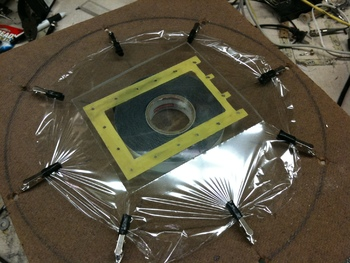
\includegraphics[width=0.5\textwidth]{images/mylar-tension-weight.png}
    \caption{A Mylar tensioning rig using weights}
    \label{f:driver:tension:weight}
\end{figure}
The other option, shown in Fig. \ref{f:driver:tension:tire}, uses a bicycle tire that is fixed to the outside of a cylinder. The Mylar is stretched over the cylinder and fixed on the bottom using adhesive tape. The tire is then inflated until the desired stretching has been achieved. A discussion on this method can be found on the head-fi thread\footnote{\url{http://www.head-fi.org/t/498292/my-diy-electrostatic-headphones/1095#post_9907534}}.
\begin{figure}[htb]
    \centering
    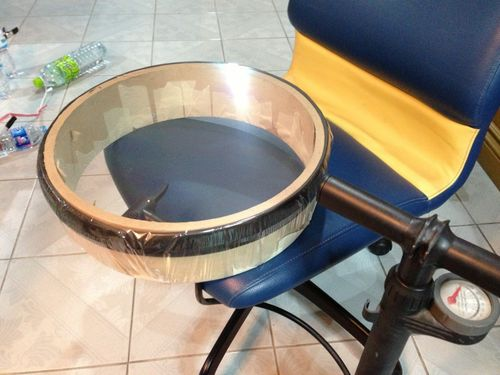
\includegraphics[width=0.5\textwidth]{images/mylar-tension-tire.png}
    \caption{A Mylar tensioning rig using an inflatable tire}
    \label{f:driver:tension:tire}
\end{figure}
%\url{http://www.head-fi.org/t/498292/my-diy-electrostatic-headphones/720#post_9217468} -> Orpheus clone tensioning; weights should be larger between 0.8 and 1.0 kg. Preferred option
As mentioned above we will use the method with the weights in the following. In our case we used 8 weights with 1 kg each and attach it to the Mylar. A picture of our improvised jig can be seen in Fig. \ref{f:driver:tension:weight:2}. We used a pan and placed a thick sheet of paper on it in order to provide a flat base for the Mylar to lie on. Gaffer tape was used to attach the weights equally around the outside. Next, we put our two back spacers on the Mylar and drew the outline onto the Mylar. Gluing both spacers at the same time ensures that the tension is the same on both sides. The spacers were then removed and both the spacer and their outline on the Mylar were covered with a thin layer of UHU Greenit. This is a contact cement or synthetic rubber glue, alternatives include UHU Por, 3M 4693. The glue is allowed to dry for 15 minutes, after which the spacers are placed onto the Mylar and pressed firmly onto them. We actually used a rolling pin to increase the pressure and thus the glueing strength\footnote{\url{http://www.head-fi.org/t/498292/my-diy-electrostatic-headphones/1215#post_10400583}}.
\begin{figure}[htb]
    \centering
    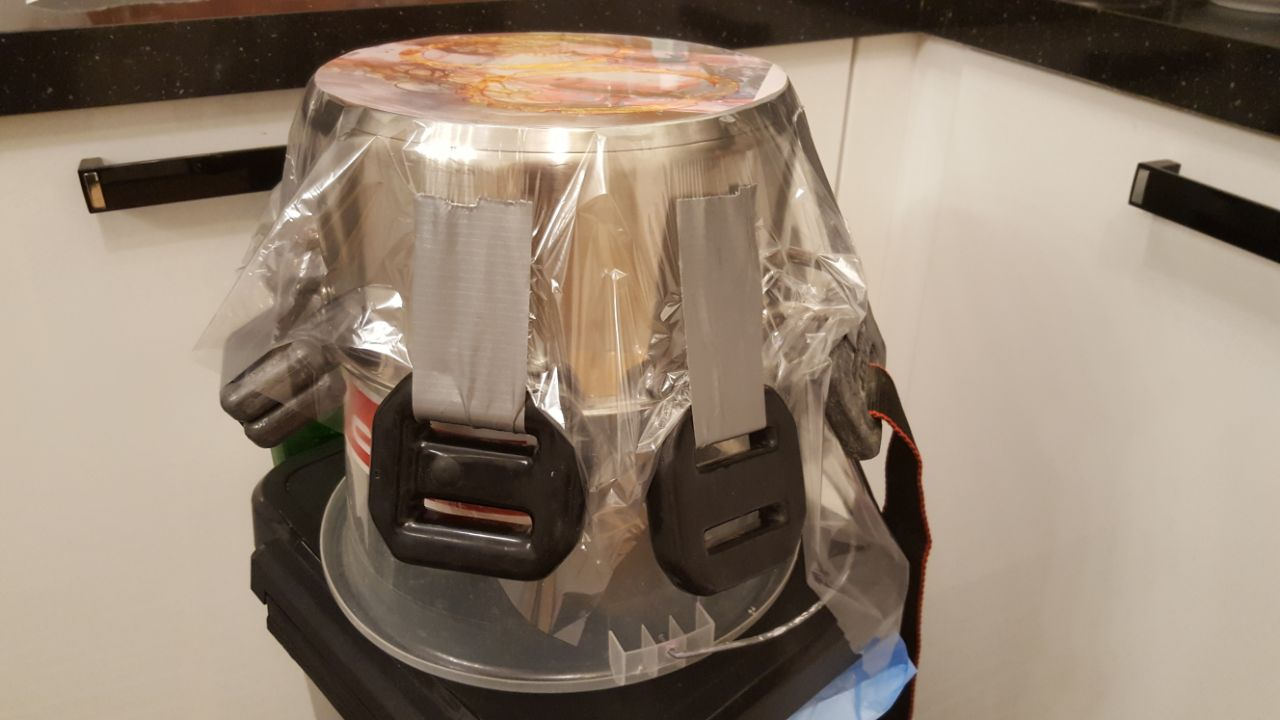
\includegraphics[width=0.5\textwidth]{images/mylar-tension-weight-2.png}
    \caption{Our Mylar tensioning rig using weights}
    \label{f:driver:tension:weight:2}
\end{figure}
After this, the weights can be removed and the excess Mylar can be cut away from the spacers. Note that it is very important to not have any Mylar overlap the edge of the spacer. We used a small scissor and then went around the edges with an old soldering iron to ensure this. After completing this step the spacers can be knocked on the side of a table to check whether the sound of both diaphragms is similar. If not, a  hot air gun can be used to loosen the tension of a diaphragm.

An idea on how to identify the correct tension of the diaphragm by checking the free-air resonance frequency (should be between 100 and 200 Hz) using a white noise generator on one side and a microphone on the other was also mentioned in the thread\footnote{\url{http://www.head-fi.org/t/498292/my-diy-electrostatic-headphones/1770#post_11440100}}, but we did not try this.

Note, while this step sounds easy, it is actually the most difficult one to get right and has probably the most significant impact on the sound of your headphones. Because of this is makes sense to actually produce a few extra back spacers to try different configurations. Alternatively, UHU Greenit can be removed from the spacers using Acetone, so a new attempt can be made.

%Tension is sufficient if wrinkles on the Mylar vanish during the procedure, corresponding to about 0.5\% of displacement.

\subsection{Coating the diaphragm}
As Mylar is not conductive an additional coating is required so that it can be charged. It basically should act as if it was a capacitor, so a coating that is conductive and has a high resistivity is ideal. Coating agents mentioned in the thread are:
\begin{enumerate}
    \item Staticide 6300 (anti-static cleaner for monitors)
    \item Licron antistatic spray
    \item Swash Floor cleaner
\end{enumerate}
In our case we simply bought a anti-static spray for computer monitors, which worked without any issues. Coating is achieved by applying a small drop of the coating agent onto the diaphragm and then spreading it with a sponge or microfibre cloth (lint free). The coating only happens on one side of the diaphragm namely the side pointing away from the spacer. It should be ensured that the coating also happens on the part of the diaphragm that is above the spacer, i.e. all the way to the edge. After the coating has dried the surface can be cleaned again with a dry lint free cloth. It is advisable to check the surface before the assembly to ensure that there is no dust on it. Otherwise pressurized air or masking tape can be used to clean the diaphragm.

Diyaudio.com also has a thread about coating\footnote{\url{http://www.diyaudio.com/forums/planars-exotics/109789-esl-diaphragm-coating.html}}.

\subsection{Cable}
The cable that connects the headphone with the step up transformer consists of three about 3m long litz wires ($0.14mm^2$)that were braided together. One side was soldered directly onto the stators and one spacer whereas the other side was fitted with banana plugs to connect the headphones to the transformer.

While this might not be the perfect solution in terms of elegance and signal transmission it was a inexpensive and functional way to make the headphones sing.

Alternatives include replacement cables for KOSS headphones. Apparently an extension cable for the ESP-950 headphone should do the trick. \footnote{\url{https://www.head-fi.org/threads/my-diy-electrostatic-headphones.498292/page-51#post-9325470}}

%Cables should be doubly insulated to withstand the high voltage. DIN plugs are used by many for electrostatic headphones but it might not be safe due to the high voltages, same for XLR. Ribbon cables rated for high voltages are recommended.
%\begin{enumerate}
%    \item Cable building (low capacitance)
%    \item Connector building: need 6 pins ideally (3 for each side, for front and rear stator as well as one for the diaphragm DC voltage)
%\end{enumerate}

\subsection{Assembly}
\label{s:driver:assembly}
Before assembling the driver a dust protector needs to be built using the 1 mm spacer made from FR4 and a 1 $\mu m$ Mylar film. The Mylar is crumpled by hand and then slightly stretched using masking tape on a flat surface. We then follow the same procedure as for the diaphragm, i.e. putting glue on both the spacer and the Mylar, letting it dry and then pressing the two firmly together. The crumpling of the Mylar should ensure that this film is acoustically transparent but keeps dust out of the driver. The slight stretching is needed so that it doesn't touch the spacer. The dust protection is only between the ear and the driver as the coated side of the diaphragm is also towards the ear. Because of this, no dust protection is required on the outside.

As we chose to have no connector directly at the headphone, we soldered the cables directly onto the two stators and the 0.5 mm front spacer without the diaphragm. Then the conducting side of the two stators was sprayed with (in our case black) acrylic spray to insulate them. This avoids arching once the stators and diaphragm are charged.

Afterwards the driver can be assembled. See Fig. \ref{f:driver:assembly:arrangement} for a visual representation of the arrangement of the different parts. The part furthest away from the ear is the stator with negative wire with the acrylic covered copper side pointing towards the ear. This is followed by the spacer with the diaphragm where the side with the diaphragm and the coating points towards the ear. Next, the front spacer is added with its copper side pointed away from the ear so that an electric connection between the diaphragm and the front spacer with the cable is made. The remaining stator is then placed onto the spacer with the acrylic covered copper side pointing away from the ear. Finally, the dust spacer is placed on the assembly with the crumpled Mylar pointing towards the ear to complete the driver.

\begin{figure}[htb]
    \centering
    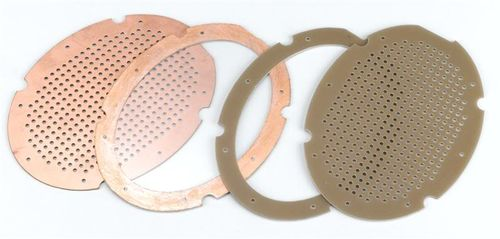
\includegraphics[width=0.5\textwidth]{images/arrangement.png}
    \caption{Arrangement and orientation of stators and spacers (missing the dust protection spacer and film)}
    \label{f:driver:assembly:arrangement}
\end{figure}

To perform some tests we used some clothespins to keep the driver together. Be careful when running tests with the driver outside the enclosure as nearly all parts will be charged. The driver can be tested by hooking it up to the amp and leave it as is for 3 to 4 hours without playing any music. The diaphragm should not be sucked to one side during this. It is also easy to hear any arching that occurs due to dust or other mistakes in the production. Sometimes it is easy to see where the arching occurs and it is usually easy to correct the cause (by using pressurized air or sanding the corners). After testing and before the driver is disassembled, e.g. for correcting something, it is advisable to connect all three wires to ground in order to allow the parts to discharge.

%\subsection{TODO}
%\begin{enumerate}
%    \item What does it mean to bias the headphone for a certain voltage?
%    \item What is used to coat the diaphragm? Coating is done with a wet sponge maybe.
%    \item How much does the Mylar need to be stretched ($< 1\%$)? About 0.5 \% seems reasonable
%    \item How to do accurate etching and what chemicals should be used? FeCl or HCl are options
%    \item How can the surface resistance of the diaphragm be measures? Simply measure at opposite sides? Check multimeter capabilities as it might not be able to measure resistance in the GOhm range. Try to find alternative ways of measuring resistance if that is the case. Resistance should be around 10 - 100 MOhm per square (cm ?). \url{https://dannyelectronics.wordpress.com/2016/01/28/the-nano-ammeter-you-already-have/} shows a way to measure small currents
%\end{enumerate}
%
%\subsection{Potential improvements}
%\begin{enumerate}
%    \item Drill holes with two different sizes to get a larger hole to surface area ratio
%    \item A space filling curve could be used to further reduce the copper on the stators
%\end{enumerate}

\section{Building the enclosure}
\label{s:enclosure}

Since we were already using a CNC machine to manufacture the drivers we opted for the same toolchain to create the enclosure. As wood is a common material in enclosure construction we decided to use it as well. We again designed the enclosure as a 2.5-D shape using Inkscape. The Gcode was created using \url{www.makercam.com} similarly to the driver. To machine the enclosure we used a 6mm and a 2mm 2-flute end mill.

\begin{figure}[htb]
    \centering
    \begin{subfigure}[b]{0.24\textwidth}
        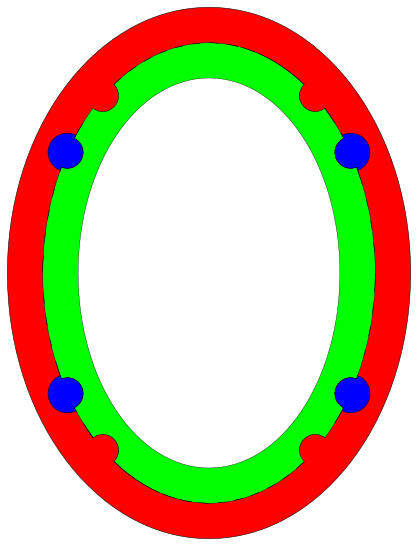
\includegraphics[width=\textwidth]{images/encasing_back_height_map.png}
        \caption{Back enclosure (red: 10mm, blue: 8mm, green: 4mm)}
        \label{f:enclosure:back}
    \end{subfigure}
    \begin{subfigure}[b]{0.24\textwidth}
        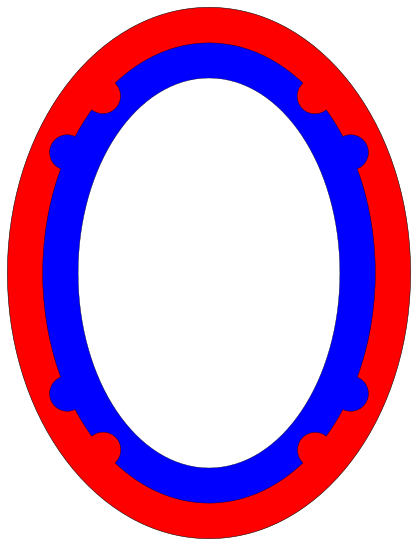
\includegraphics[width=\textwidth]{images/encasing_front_height_map.png}
        \caption{Front enclosure (red: 2mm, blue: 4mm)}
        \label{f:enclosure:front}
    \end{subfigure}
    \begin{subfigure}[b]{0.24\textwidth}
        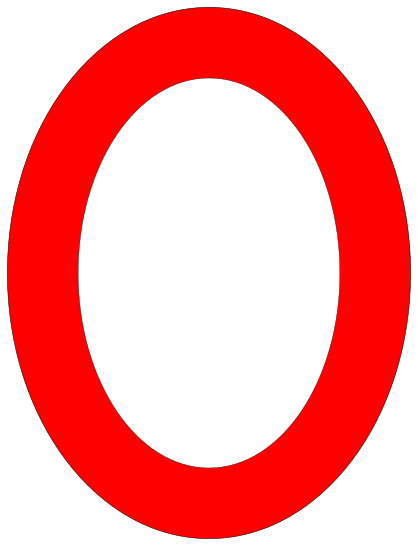
\includegraphics[width=\textwidth]{images/pad_height_map.png}
        \caption{Pad ring (red: 4mm)}
        \label{f:enclosure:pad}
    \end{subfigure}
    \caption{Height maps of all enclosure components}
    \label{f:enclosure:components}
\end{figure}

All three wooden components of the enclosure can be seen in Fig. \ref{f:enclosure:components}. The back enclosure is the part furthest away from the ear and has a maximum thickness of 10 mm (see Fig. \ref{f:enclosure:back}) and is responsible for housing the driver. The four blue circles and the four red half circles were put into place to provide a fixed space for the driver to sit in. However, as our opening is elliptic, the driver cannot move anyways, so this was not really necessary. The second reason for this was to provide space for up to 8 screws to hold everything together. In the end we only used four screws which were drilled through the center of the blue circles. Our biggest mistake when making the enclosures was to not allow for any space between the driver and the enclosure. In a perfect world, everything would have fit, but in reality it would make sense to leave a bit of room, e.g. 0.5 mm. We also did not include any space for the cables at the bottom of the back enclosure. This was later added manually, but ideally, we would have added this at this stage already as it would make everything a lot cleaner.

The front enclosure is fairly straightforward and is machined from 4 mm thick wood. It's main task is to keep the driver inside the back enclosure. Again, because we machined it to perfect precision we needed to do quite a bit of sanding to eventually get it to fit. Since we are machining wood, the mill actually compresses the wood and a perfect fit is not attainable.

Finally, the last part is the pad ring. This ring will sit inside the ear pad and we use it to glue the leather of the pad onto it and provide screw holes for the connection with the enclosure.

After milling these components for each side, we sanded them down to make sure that they fit together and get a smooth finish. We assembled the three parts together and used a 2 mm drill to create four screw holes (as noted above, through the blue circles in the back encasing). Additional holes where drilled into the side of the back enclosure to accommodate the wires from the headband, see below. We then applied some transparent wood glaze and let the pieces dry. Unfortunately, the glaze was quite thick, so it did not look very clean. For the next iteration we will probably use a different finish (e.g. wax or oil).

% Wooden enclosures are potentially problematic as they can attract moisture which can cause electrical leakage. Sennheiser uses varnish on the outside of their wooden cups but none on the inside. It is possible to use a plastic O-ring to avoid direct contact between the wood and the driver.

\section{Building the headband}
\label{s:headband}
TODO-BB

\url{http://www.head-fi.org/t/498292/my-diy-electrostatic-headphones/675#post_8943826}

Headband can be made out of a metal ruler and then covered with leather \url{http://www.head-fi.org/t/498292/my-diy-electrostatic-headphones/2385#post_13037825}.

\section{Building the earpads}
\label{s:pads}
The earpads should be thick enough so that the bass is powerful and deep enough.
\begin{figure}
\centering
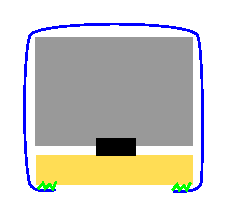
\includegraphics[width=0.3\textwidth]{images/earpad.pdf}
\caption{Earpad cut-through; materials: wooden pad ring (yellow), foam (grey), screw nut (black), artificial leather (blue), contact cement (green)}
\label{f:pads:cut}
\end{figure}
The earpad is based on a wooden ellipse with 4mm thickness that was also manufactured using the CNC. After we had the full enclosing together we put the front and the back of the enclosing together with this ellipse to drill four holes for the assembly. The screw nuts were glued to the inside of the ellipse using copious amounts of epoxy. A schematic of the earpad can be seen in Fig. \ref{f:pads:cut}. After the glue has hardened (see your glue for the time, for ours it was about 24h) we loosened the screws and disassembled everything. The next step consisted of cutting the same ellipse from acoustic foam with 3cm thickness.

The leather cover is made from a thin and stretchy synthetic leather. It's made of two parts, a rectangular one with dimension 4 x 32 cm and an elliptic one which is of the same size as the wooden ellipse of the pad plus 1 cm inside and 3 cm on the outside. The rectangular patch is sewn on the inside of the ellipse and then it's wrapped over the foam and the wooden pad connector. The leather is glued to the wood using the contact cement that was also used to glue the diaphragm to the spacers. Finally, we also glued a mesh to the wood so that the ears cannot get in touch with the dust protector.

\begin{figure}
\centering
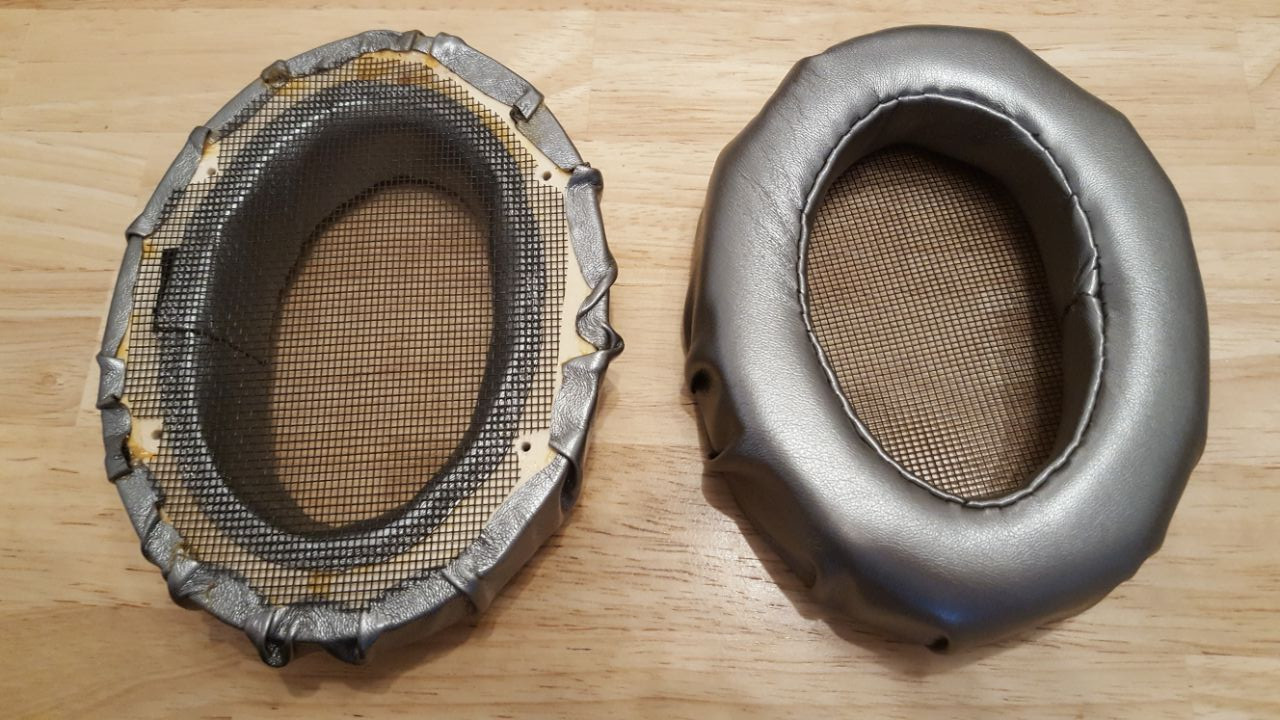
\includegraphics[width=0.7\textwidth]{images/earpads_final.jpg}
\caption{Final earpads}
\label{f:pads:final}
\end{figure}

%\subsection{Potential improvements}
%\begin{enumerate}
%    \item Material should be leather on the inside. Sennheiser HE60/90 has fabric in contact with head, leather everywhere else. This makes it more comfortable
%    \item It might be worth having harder foam on the inside as it will reduce resonances. Obviously this needs to be balanced to ensure comfort.
%    \item Is it possible to make individual ear pads? Would allow for the use of harder materials. Moving your mouth changes the geometry so one would need to be careful.
%\end{enumerate}
%Post on ear pads: \url{http://www.head-fi.org/t/498292/my-diy-electrostatic-headphones/660#post_8930271}. Inner diameter of Orpheus earpads is 45mm x 90mm.

\section{Assembly}
\label{s:assembly}

At this time pretty much everything is ready for assembly. We only made one small additional change to the back enclosure which consisted of adding a plastic net to the outside so that it was not possible to directly touch the driver. We attempted to do this by stapling the net to the inner, 4 mm high side wall, but this was quite a fiddly task. For our next iteration we will probably think about this issue beforehand to make sure that this will look smoother and is easier to assemble.

After the back enclosure was ready, we inserted the driver. This is done in the following order:

\begin{enumerate}
\item Stator with acrylic (copper) side pointing towards the ear
\item 0.5 mm spacer with membrane, which is pointing towards the ear
\item 0.5 mm Spacer with the cable and conducting copper side, which should be pointing away from the ear
\item Stator with acrylic (copper) side pointing away from the ear
\item 1 mm spacer with crumpled membrane, which is pointing towards the ear
\end{enumerate}

After threading the cable through the opening, we added the front enclosure to keep everything in place. The two enclosure parts were then connected using the four 2 mm screws. The earpad is then placed on the assembly and the four screws are driven through the pad to complete it. Finally, the headband is inserted into the holes inside of the back enclosure.

\begin{figure}[htb]
    \centering
    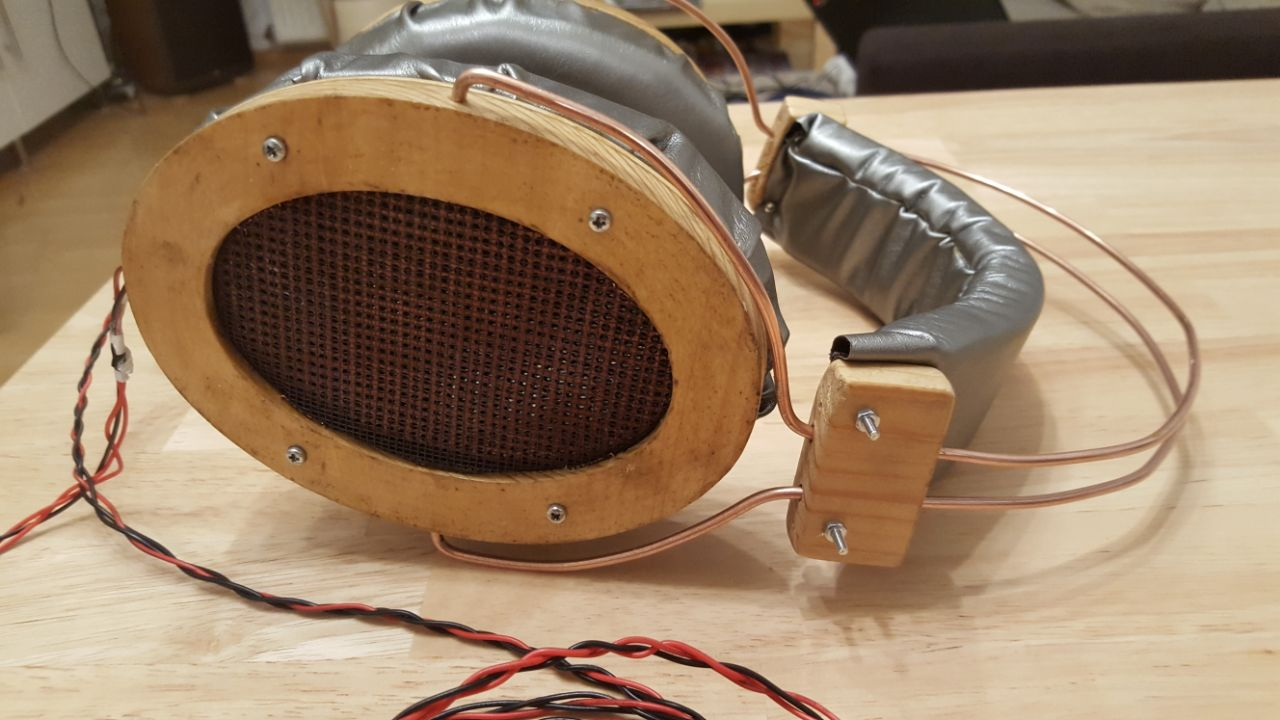
\includegraphics[width=0.95\textwidth]{images/headphones_side.jpg}
    \caption{The assembled headphones}
    \label{f:assembly:phones}
\end{figure}

\section{Amplifier}
\label{s:amp}
Due to the requirement of a continuously charged diaphragm and the high voltage requirements of the stators a dedicated amplifier is required for electrostatic headphones.
\begin{figure}[htb]
    \centering
    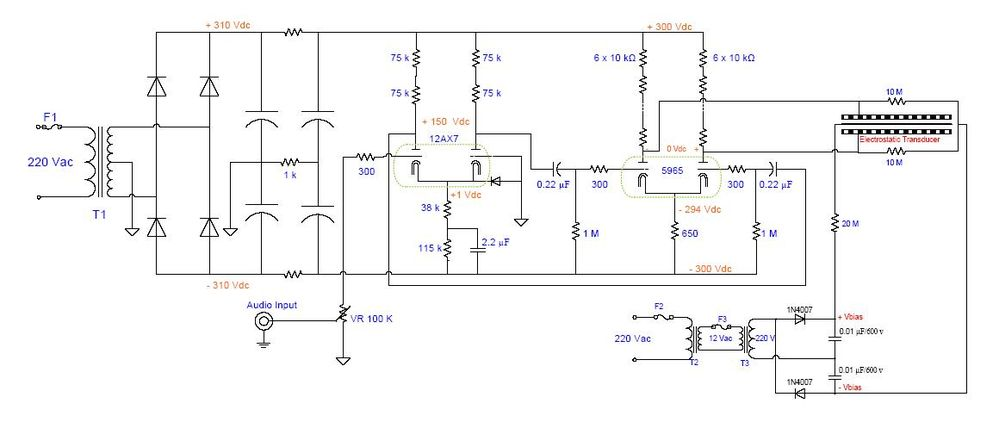
\includegraphics[width=0.5\textwidth]{images/wachara-amp.png}
    \caption{Amplifier design by Wachara C.}
    \label{f:amp:wachara}
\end{figure}
A discussion on this amplifier design can be found on Head-fi.org \footnote{\url{http://www.head-fi.org/t/498292/my-diy-electrostatic-headphones/720#post_9182523}}. However, to not make out lives too difficult we decided against building a full amplifier. Instead we opted to construct a step up transformer based on the designs of Charlie Mimbs \footnote{\url{https://jazzman-esl-page.blogspot.co.at/2010/01/update-new-toroidal-step-up.html}}.

A note of warning before we continue with the details. We will be dealing with electronic equipment in the following which can cause serious injury or death so make sure you have a good understanding of what you are doing and follow proper safety procedures.

Since we are not building a speaker we opted for a toned down version of Charlie's step up that would only lead to 580 volts at the diaphragm. A circuit diagram can be seen in Fig. \ref{f:amp:step-up} that was copied from circuitjs \footnote{\url{http://lushprojects.com/circuitjs/circuitjs.html}}.

\begin{figure}[htb]
    \centering
    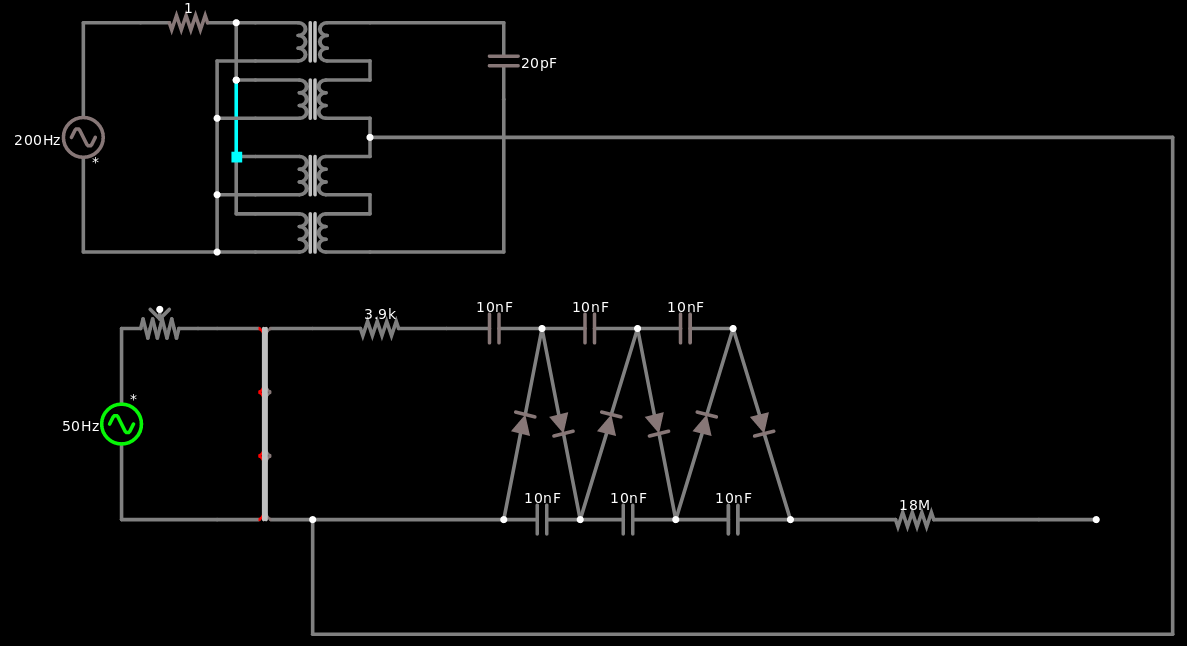
\includegraphics[width=0.7\textwidth]{images/step-up-transformer.png}
    \caption{Step up transformer: circuit diagram}
    \label{f:amp:step-up}
\end{figure}

The final step-up transformer can be seen in Fig. \ref{f:amp:step-up-real}. As can be seen, we did not put it in a nice enclosing and this will also be part of next years project. The step-up transformer is divided in three parts, the blue and yellow part are the transformers for the left and right stators, respectively. Each of these section consists of one 1 Ohm resistor and 2 audio transformers from 6 V to 230 V. The OEP transformers that we used (see Section \ref{s:materials}) were connected on the B-D and 1-4 pins. This yields a 4000k to 95k winding ratio. The two transformers are connected in series and the output side is connected to the step-up part of the transformer as can be seen in Fig. \ref{f:amp:step-up}. Note that in the circuit diagram only one of these stator sections is depicted.

\begin{figure}[htb]
    \centering
    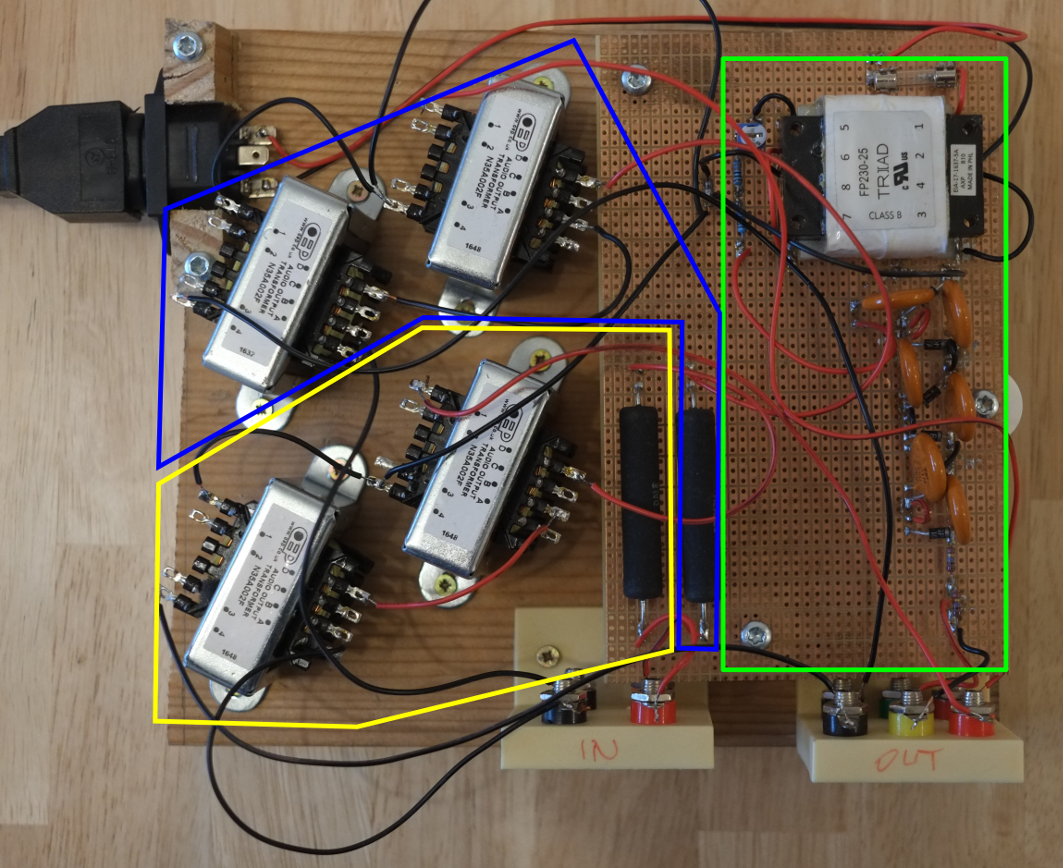
\includegraphics[width=0.95\textwidth]{images/step-up-real-top.png}
    \caption{Step up transformer from the top}
    \label{f:amp:step-up-real}
\end{figure}

The green part in Fig. \ref{f:amp:step-up-real} corresponds to the lower part in the circuit diagram (Fig. \ref{f:amp:step-up}) and is responsible for converting the 230 V, 50 Hz AC input to a 580 V DC current. The AC input was connected to the Triad power transformer including a 250mA fast blow fuse. On the output side a 3.9 kOhm resister is put before the actual step-up ladder that can be seen in the circuit diagram. This ladder consists of 6 10 nF capacitors and 6 diodes to rectify the AC current. At the end of this ladder a 18 MOhm resistor is put before the connection to the diaphragm is made. Note that we made only one step-up ladder that is connected to both left and right diaphragms.

Note that when operating the headphone its component will be charged and this charge will persist even if power to the transformer has been shut down. It is necessary to discharge all components before disassembly which can be achieved by leaving the power cord connected after shutdown and using the ground connection of the power cord. We hooked up a cable to the ground connection and discharge all outgoing ports by touching them briefly with this cable.

\begin{figure}[htb]
    \centering
    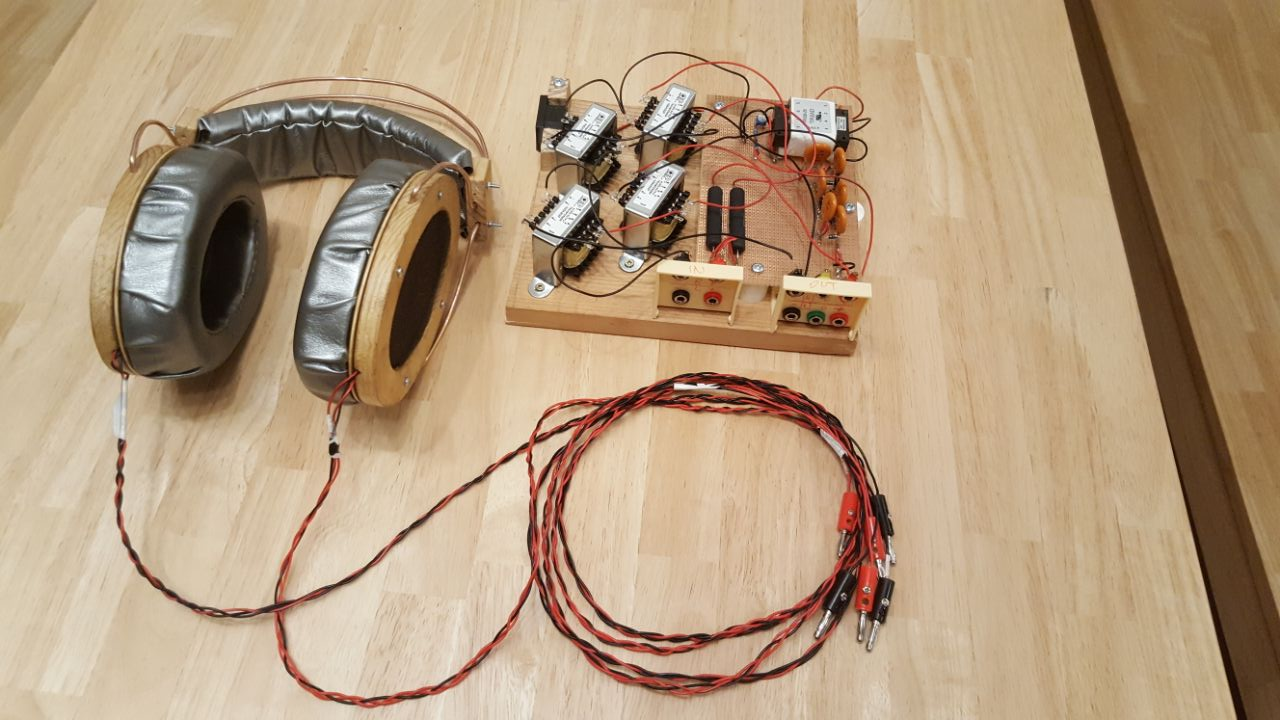
\includegraphics[width=0.95\textwidth]{images/headphones_and_amp.jpg}
    \caption{Headphones and step-up transformer}
    \label{f:amp:all}
\end{figure}

%Check if it is possible to add a voltage regulator to try out different bias voltages easily \url{http://www.head-fi.org/t/498292/my-diy-electrostatic-headphones/1560#post_10959595}.
%
%Amp safety: \url{http://www.head-fi.org/t/498292/my-diy-electrostatic-headphones/1455#post_10705917} and \url{http://www.head-fi.org/t/498292/my-diy-electrostatic-headphones/1470#post_10706261}
%
%Check design in article \cite{ww_1979} and \cite{verwaal_2011}.
%
%Turn ratio should be at least around 1:40.
%
%\url{http://www.head-fi.org/t/498292/my-diy-electrostatic-headphones/2415#post_13059527} pdf with some links and amp designs

\section{Measurements}
\label{s:measurements}

As part of the current build we did not perform any measurements and this will become a topic for the future. The head-fi thread suggests to perform measurements with and without seal. The latter should give a peak at around 200 Hz which is the free-air resonance frequency. This frequency should be lower than 150 Hz for a good bass response.

\section{What to do different in the future}
\label{s:future}

Allow for a little space between enclosing and driver.

Shrink wrapped cable with proper xlr connector and connector at the headphone. Space for the cables milled out when creating the enclosure.

Earpad made out of three pieces (2 rectangular ones and one ellipse).

Proper enclosing for the step-up transformer or even a real amplifier for electrostatic headphones. Additional cables to connect the step-up transformer to headphone amplifiers.

\subsection{Closed headphones}
\label{s:future:closed}

We did not really attempt closed headphones for this first prototype as it comes with all sorts of issues that we wanted to avoid. The biggest certainly is the damping of the noise on the outside. Materials used for damping included felt, wool or other acoustically semi-transparent materials. Some also coat the inside of the enclosure with Bitumen. But these are just some notes that we found while reading the thread on Head-Fi. More practical experience might follow in the future (or from you).

\section{Collaboration \& License}
\label{s:collab}
This work is licensed under a Creative Commons Attribution-ShareAlike 4.0 International License \footnote{\url{http://creativecommons.org/licenses/by-sa/4.0/}}. The official repository for this guide can be found on github.com \footnote{\url{https://github.com/Azrael3000/headphone-guide}}. There is an issue tracker available on this site if you do not know how to work with \LaTeX and git.

We very much jumped into this venture without prior knowledge of a lot of things that we had to tackle. Because of this there might very well be mistakes in this guide or in our approach that we are happy to learn about. So do get in touch with us if you have any remarks and want to help us improve this document. We plan to build version 2 of the headphones in 2018 and with this we will also update and improve this guide.

\begin{figure}[htb]
    \centering
    
\includegraphics[width=0.6\textwidth]{images/arno_and_benni.jpg}
    \caption{Arno and Benni, the two authors with the finished headphones}
    \label{f:collab}
\end{figure}

\section{Appendix}
\label{s:app}

\subsection{Circuit diagram for circuitjs}
\label{s:app:circuit}
This file can also be found in the resources.zip file which can be found on github.com \footnote{\url{https://github.com/Azrael3000/headphone-guide/raw/master/resoures.zip}}.
\begin{verbatim}
$ 13 0.000005 146.80153516788286 47 120 28
v 448 512 448 352 0 1 50 230 0 1.5707963267948966 0.5
c 720 352 800 352 0 1e-8 -121.77903323034391
w 608 512 608 608 0
w 608 512 768 512 0
d 768 512 800 352 1 0.805904783
d 800 352 832 512 1 0.805904783
d 832 512 880 352 1 0.805904783
d 880 352 912 512 1 0.805904783
d 912 512 960 352 1 0.805904783
d 960 352 1008 512 1 0.805904783
c 800 352 880 352 0 1e-8 -188.52952984256655
c 880 352 960 352 0 1e-8 -148.45206709826482
c 768 512 832 512 0 1e-8 -188.38552969850758
c 832 512 912 512 0 1e-8 -148.28294550190276
c 912 512 1008 512 0 1e-8 -133.83898987162684
r 1008 512 1216 512 0 18000000
w 1216 512 1264 512 0
w 608 608 1328 608 0
v 416 96 416 288 0 1 200 6 0 0 0.5
T 560 96 656 112 0 4 20 -0.0002165438913044398 0.000008783616360946498 0.999
T 560 176 656 144 0 4 20 0.00021654389130444608 -0.000008783616360946477 0.999
T 560 240 656 208 0 4 20 0.00021654389130505795 -0.00000878361636097594 0.999
T 560 288 656 256 0 4 20 0.00021654389130505323 -0.000008783616360975917 0.999
w 656 128 656 144 0
w 656 240 656 256 0
r 544 96 464 96 0 1
w 544 96 560 96 0
w 544 208 560 208 0
w 544 144 560 144 0
w 544 208 544 256 0
w 544 256 560 256 0
w 544 208 544 144 0
w 544 144 544 96 0
w 560 128 528 128 0
w 528 128 528 176 0
w 528 176 560 176 0
w 528 176 528 240 0
w 528 240 560 240 0
w 560 288 528 288 0
w 528 288 528 240 0
w 416 288 528 288 0
w 464 96 416 96 0
w 1328 608 1328 192 0
w 1328 192 656 192 0
w 656 208 656 192 0
w 656 192 656 176 0
w 656 288 768 288 0
w 768 288 768 160 0
w 656 96 768 96 0
c 768 96 768 160 0 2e-11 -328.31758099807905
T 608 352 528 192 0 2 1 -4.752600223090209e-16 -0.18138620921599558 0.999
r 608 352 720 352 0 3900
w 448 512 528 512 0
174 448 352 512 352 0 1000 0.5 Resistance
w 512 352 528 352 0
o 16 64 0 2083 1280 0.00009765625 0 -1 0
o 49 64 0 2083 1280 0.0001953125 1 -1 0
o 51 64 0 2083 5 0.0015625 2 -1 0
o 1 64 0 2083 320 0.0015625 3 -1 0
o 3 64 0 2083 640 0.0015625 4 -1 0
o 54 64 0 2083 640 0.4 5 -1 0
\end{verbatim}


\bibliographystyle{plain}
\bibliography{main}

\end{document}
